\documentclass[a4paper,11pt]{article}

% =========================================================
% PACKAGES & CONFIGURATION
% =========================================================
\usepackage[utf8]{inputenc}
\usepackage[T1]{fontenc}
\usepackage[margin=1in, bottom=1.2in]{geometry}
\usepackage{xcolor}
\usepackage{graphicx}
\usepackage{titlesec}
\usepackage{fancyhdr}
\usepackage{tcolorbox}
\usepackage{fontawesome5} % For icons
\usepackage{booktabs}
\usepackage{tabularx}
\usepackage{multirow}
\usepackage{tikz}
\usepackage{float}
\usepackage{hyperref}
\usepackage{enumitem}

\usetikzlibrary{shapes.geometric, arrows, positioning}
\tcbuselibrary{skins, breakable}

% =========================================================
% WARLOCK STUDIO BRANDING COLORS (From Source Code)
% =========================================================
\definecolor{WarlockBg}{HTML}{0A0A0A}       % Main Background
\definecolor{WarlockRed}{HTML}{D41C1C}      % Accent Red
\definecolor{WarlockGold}{HTML}{FDEF2F}     % Accent Gold
\definecolor{WarlockDark}{HTML}{303030}     % Widget Background
\definecolor{WarlockText}{HTML}{FFFFFF}     % White Text
\definecolor{WarlockGray}{HTML}{B5B4B4}     % Secondary Text


% Header and Footer
\pagestyle{fancy}
\fancyhf{}
\renewcommand{\headrulewidth}{0pt}
\renewcommand{\footrulewidth}{2pt}
\renewcommand{\footrule}{\hbox to\headwidth{\color{WarlockRed}\leaders\hrule height \footrulewidth\hfill}}

\fancyhead[R]{\textbf{\textcolor{WarlockDark}{Warlock-Studio v5.1}}}
\fancyhead[L]{\textcolor{WarlockGray}{User Manual}}
\fancyfoot[C]{\thepage}
\fancyfoot[R]{\includegraphics[height=0.8cm]{logo.png}} % Logo at footer

% Section Styling
\titleformat{\section}
{\color{WarlockRed}\normalfont\Large\bfseries\uppercase}
{\thesection}{1em}{}[{\titlerule[1pt]}]

\titleformat{\subsection}
{\color{WarlockDark}\normalfont\large\bfseries}
{\thesubsection}{1em}{}

% Custom Boxes for Information grouping
\newtcolorbox{infobox}[1]{
  colback=WarlockDark!10!white,
  colframe=WarlockDark,
  fonttitle=\bfseries,
  title=#1,
  arc=0mm,
  boxrule=1pt,
  leftrule=4pt
}

\newtcolorbox{warningbox}[1]{
  colback=red!5!white,
  colframe=WarlockRed,
  fonttitle=\bfseries,
  title=\faExclamationTriangle\ #1,
  arc=0mm,
  boxrule=1pt,
  leftrule=4pt,
  coltitle=white
}

\newtcolorbox{tipbox}[1]{
  colback=WarlockGold!10!white,
  colframe=orange!80!black,
  fonttitle=\bfseries,
  title=\faLightbulb\ #1,
  arc=0mm,
  boxrule=1pt,
  leftrule=4pt,
  coltitle=black
}

% Hyperlink Setup
\hypersetup{
    colorlinks=true,
    linkcolor=WarlockRed,
    filecolor=magenta,
    urlcolor=blue,
    pdftitle={Warlock-Studio Manual},
}

% =========================================================
% DOCUMENT CONTENT
% =========================================================

\begin{document}

% --- COVER PAGE ---
\begin{titlepage}
    \begin{center}
        \vspace*{2cm}
        \includegraphics[width=0.4\textwidth]{logo.png}\\[1cm]

        {\Huge \textbf{WARLOCK-STUDIO}}\\[0.5cm]
        {\Large \textit{AI Upscaling \& Interpolation Suite}}\\[0.2cm]
        {\large Version 5.1}

        \vspace{2cm}

        \begin{tcolorbox}[colback=WarlockDark, colframe=WarlockRed, width=0.8\textwidth, arc=2mm]
            \centering \textcolor{white}{\textbf{\Large USER OPERATING MANUAL}}
        \end{tcolorbox}

        \vfill

        \textbf{Developed by Ivan-Ayub97}\\
        \today

    \end{center}
\end{titlepage}

\tableofcontents
\newpage

% ---------------------------------------------------------
% SECTION 1: INTRODUCTION
% ---------------------------------------------------------
\section{Introduction}
Warlock-Studio is a comprehensive GUI application designed for AI-driven image and video enhancement. It integrates state-of-the-art neural networks to perform Upscaling, Denoising, Face Restoration, and Frame Interpolation.

Built on Python, CustomTkinter, and ONNX Runtime, Warlock-Studio optimizes hardware resources (CPU and GPU) to deliver great results.

\begin{infobox}{System Requirements}
\begin{itemize}
    \item \textbf{OS:} Windows 10/11 (x64)
    \item \textbf{RAM:} Minimum 8GB (16GB+ recommended)
    \item \textbf{GPU:} NVIDIA (CUDA), AMD/Intel (DirectML), or CPU (Slow fallback)
    \item \textbf{Dependencies:} FFmpeg (included in assets), Visual C++ Redistributable.
\end{itemize}
\end{infobox}

% ---------------------------------------------------------
% SECTION 2: INTERFACE & USAGE
% ---------------------------------------------------------
\section{Interface Overview & Usage}
The interface is divided into functional blocks designed for a linear workflow: \textit{Load $\rightarrow$ Configure $\rightarrow$ Process}.

\subsection{1. Input Section}
Located on the left side (or top, depending on layout), this area handles file ingestion.
\begin{itemize}
    \item \textbf{Drag \& Drop:} You can drag images or videos directly onto the window.
    \item \textbf{Manual Select:} Clicking the button opens a file dialog.
    \item \textbf{File List:} Selected files appear in a scrollable list showing resolution, duration, and calculated output resolution based on current settings.
\end{itemize}

\subsection{2. AI Configuration}
This is the core control panel.
\begin{description}
    \item[AI Model:] Selects the neural network architecture (see Chapter 3).
    \item[AI Multithreading:] Controls how many frames are processed simultaneously.
    \begin{itemize}
        \item \textit{Recommendation:} Set to "2 threads" for mid-range GPUs. Use "OFF" (1 thread) for high-resolution upscaling (4K) to save VRAM.
    \end{itemize}
    \item[Frame Generation (RIFE):] Only active when RIFE models are selected. Interpolates frames to increase smoothness (e.g., 30fps $\rightarrow$ 60fps).
\end{description}

\subsection{3. Hardware & Performance}
\begin{itemize}
    \item \textbf{GPU Selection:} Choose specific GPU or "Auto".
    \item \textbf{VRAM Limiter:} \textbf{Crucial Setting.} This defines the tile size for processing.
    \begin{itemize}
        \item \textit{Integrated Graphics:} Set to 2GB or lower.
        \item \textit{Dedicated GPU (e.g., RTX 3060):} Set to match your card's VRAM (e.g., 6GB-8GB).
    \end{itemize}
\end{itemize}

\begin{tipbox}{Tiling Technology}
Warlock-Studio uses "Tiling". If an image is too large for VRAM, it splits the image into small squares, processes them, and merges them back. The \textbf{VRAM Limiter} controls the size of these squares.
\end{tipbox}

\subsection{4. Resolution Control}
\begin{itemize}
    \item \textbf{Input Resolution \%:} Downscales the image \textit{before} AI processing. Useful for speeding up 4K video processing (e.g., set to 50\%).
    \item \textbf{Output Resolution \%:} Downscales the image \textit{after} AI processing.
\end{itemize}

\subsection{5. Output Settings}
\begin{itemize}
    \item \textbf{Image Ext:} PNG (Lossless), JPG (Fast), BMP/TIFF (Uncompressed).
    \item \textbf{Video Ext:} MP4, MKV, AVI, MOV.
    \item \textbf{Video Codec:}
    \begin{itemize}
        \item \textbf{x264/x265:} CPU Encoding (High quality, slow).
        \item \textbf{NVENC:} NVIDIA Hardware (Fast).
        \item \textbf{AMF:} AMD Hardware.
        \item \textbf{QSV:} Intel Hardware.
    \end{itemize}
\end{itemize}

% ---------------------------------------------------------
% SECTION 3: AI MODELS EXPLAINED
% ---------------------------------------------------------
\newpage
\section{AI Models Library}
Warlock-Studio includes varied models optimized for specific scenarios. Use this table to choose the right tool.

\begin{table}[h!]
\centering
\renewcommand{\arraystretch}{1.3}
\begin{tabularx}{\textwidth}{|l|l|X|}
\hline
\rowcolor{WarlockDark} \textcolor{white}{\textbf{Category}} & \textcolor{white}{\textbf{Model Name}} & \textcolor{white}{\textbf{Best Use Case}} \\ \hline
\multirow{2}{*}{\textbf{Denoising}} & IRCNN\_Mx1 & Removing grain/noise without changing resolution. Fast. \\
 & IRCNN\_Lx1 & Heavier denoising for very grainy sources. \\ \hline
\multirow{2}{*}{\textbf{Anime / Art}} & RealESR\_Animex4 & \textbf{Best for Cartoons/Anime.} Removes compression artifacts and sharpens lines. \\
 & RealESR\_Gx4 & General purpose fast upscaling. \\ \hline
\multirow{4}{*}{\textbf{Realistic}} & BSRGANx4 & \textbf{Best for Real World video.} Adds texture and realistic details. \\
 & BSRGANx2 & 2x version of above. Slightly faster. \\
 & RealESRGANx4 & Good balance between sharpness and texture. \\
 & RealESRNetx4 & Smoother look, less texture hallucination. \\ \hline
\textbf{Faces} & GFPGAN & \textbf{Face Restoration.} Miraculous recovery of blurry/small faces. \\ \hline
\textbf{Interpolation} & RIFE / Lite & Increasing Frame Rate (30$\rightarrow$60fps). Creates intermediate frames. \\ \hline
\end{tabularx}
\caption{Warlock-Studio Model Reference Guide}
\end{table}

\subsection*{When NOT to use certain models:}
\begin{itemize}
    \item Do \textbf{not} use \textit{RealESR\_Animex4} on realistic photos; it will make skin look like plastic (oil painting effect).
    \item Do \textbf{not} use \textit{GFPGAN} on non-human subjects or high-quality faces (it might alter facial features slightly).
\end{itemize}

% ---------------------------------------------------------
% SECTION 4: WORKFLOW DIAGRAMS
% ---------------------------------------------------------
\section{Process Workflows}

\subsection{Video Upscaling Pipeline}
Understanding the internal process helps in troubleshooting speed issues.

\vspace{0.5cm}

\begin{center}
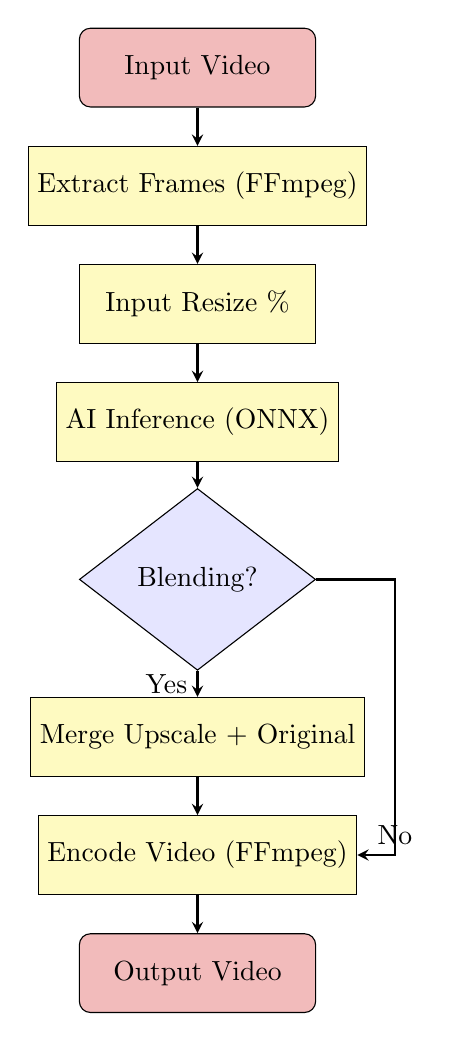
\begin{tikzpicture}[node distance=1.5cm]
    \tikzstyle{startstop} = [rectangle, rounded corners, minimum width=3cm, minimum height=1cm,text centered, draw=black, fill=WarlockRed!30]
    \tikzstyle{process} = [rectangle, minimum width=3cm, minimum height=1cm, text centered, draw=black, fill=WarlockGold!30]
    \tikzstyle{decision} = [diamond, minimum width=3cm, minimum height=1cm, text centered, draw=black, fill=blue!10]
    \tikzstyle{arrow} = [thick,->,>=stealth]

    \node (in) [startstop] {Input Video};
    \node (extract) [process, below of=in] {Extract Frames (FFmpeg)};
    \node (resize1) [process, below of=extract] {Input Resize \%};
    \node (ai) [process, below of=resize1] {AI Inference (ONNX)};
    \node (blend) [decision, below of=ai, yshift=-0.5cm] {Blending?};
    \node (merge) [process, below of=blend, yshift=-0.5cm] {Merge Upscale + Original};
    \node (encode) [process, below of=merge] {Encode Video (FFmpeg)};
    \node (out) [startstop, below of=encode] {Output Video};

    \draw [arrow] (in) -- (extract);
    \draw [arrow] (extract) -- (resize1);
    \draw [arrow] (resize1) -- (ai);
    \draw [arrow] (ai) -- (blend);
    \draw [arrow] (blend) -- node[anchor=east] {Yes} (merge);
    \draw [arrow] (blend.east) -- ++(1,0) |- node[anchor=south] {No} (encode.east);
    \draw [arrow] (merge) -- (encode);
    \draw [arrow] (encode) -- (out);

\end{tikzpicture}
\end{center}

% ---------------------------------------------------------
% SECTION 5: TROUBLESHOOTING
% ---------------------------------------------------------
\newpage
\section{Troubleshooting & Error Codes}

The integrated console (bottom of the app) provides real-time logs. Here are common errors and fixes.

\subsection{Common Runtime Errors}

\begin{table}[h!]
\centering
\begin{tabularx}{\textwidth}{|l|X|}
\hline
\rowcolor{WarlockRed} \textcolor{white}{\textbf{Error / Symptom}} & \textcolor{white}{\textbf{Solution}} \\ \hline
\textbf{CUDA / Out of Memory} & The AI model requires more VRAM than available. \newline \textbf{Fix:} Lower the "GPU VRAM" setting (e.g., set to 2). Lower "AI Multithreading" to OFF. \\ \hline
\textbf{FFmpeg not found} & The application cannot process video/audio. \newline \textbf{Fix:} Ensure \texttt{ffmpeg.exe} is in the \texttt{Assets/} folder. \\ \hline
\textbf{Gray/Black Output} & Often caused by incompatible Video Codecs. \newline \textbf{Fix:} Switch output codec to \texttt{x264} (Software) or check GPU driver updates. \\ \hline
\textbf{Process Stops Immediately} & File path issue. \newline \textbf{Fix:} Avoid special characters or emojis in filenames/folders. Move files to a simple path like \texttt{C:/Upscale/}. \\ \hline
\textbf{DLL Load Failed} & Missing Visual C++ dependencies. \newline \textbf{Fix:} Install latest MSVC Redistributable. \\ \hline
\end{tabularx}
\end{table}

\begin{warningbox}{Checkpoint Recovery}
If the app crashes during a long video upscale, \textbf{do not delete the temporary folder}. Warlock-Studio will detect the processed frames and resume from where it left off automatically upon restarting the same job.
\end{warningbox}

\subsection{Performance Tuning Tips}
\begin{itemize}
    \item \textbf{Slow Speed?} Ensure "Process Priority" in Preferences is set to "High". Check if you are using CPU instead of GPU (Console will say \texttt{CPUExecutionProvider}).
    \item \textbf{Low Quality?} Try disabling "Blending" (set to OFF). Increase "Input Resolution \%" to 100.
    \item \textbf{Glitchy Video?} If using Interpolation (RIFE), scene changes might look weird. This is a limitation of current AI flow generation.
\end{itemize}

% ---------------------------------------------------------
% SECTION 6: PREFERENCES
% ---------------------------------------------------------
\section{Preferences Menu}
Accessible via the \faCog\ icon in the top right.

\begin{itemize}
    \item \textbf{App Theme:} Switch between Dark/Light modes.
    \item \textbf{ONNX Provider:} Force specific backend (CUDA vs DirectML). \textit{Auto} is recommended.
    \item \textbf{Clean Temp Files:} Removes leftover \texttt{.tmp} files and frame folders from crashed sessions.
    \item \textbf{Extended Logging:} Enables detailed debug logs for error reporting.
\end{itemize}

\vspace{2cm}
\begin{center}
    \textit{Warlock-Studio is an open-source tool. \\ Thank you for using it.}
\end{center}

\end{document}
